\chapter{Anexo I: Árbol de Problema }

\begin{figure}[h]
	\begin{center}
		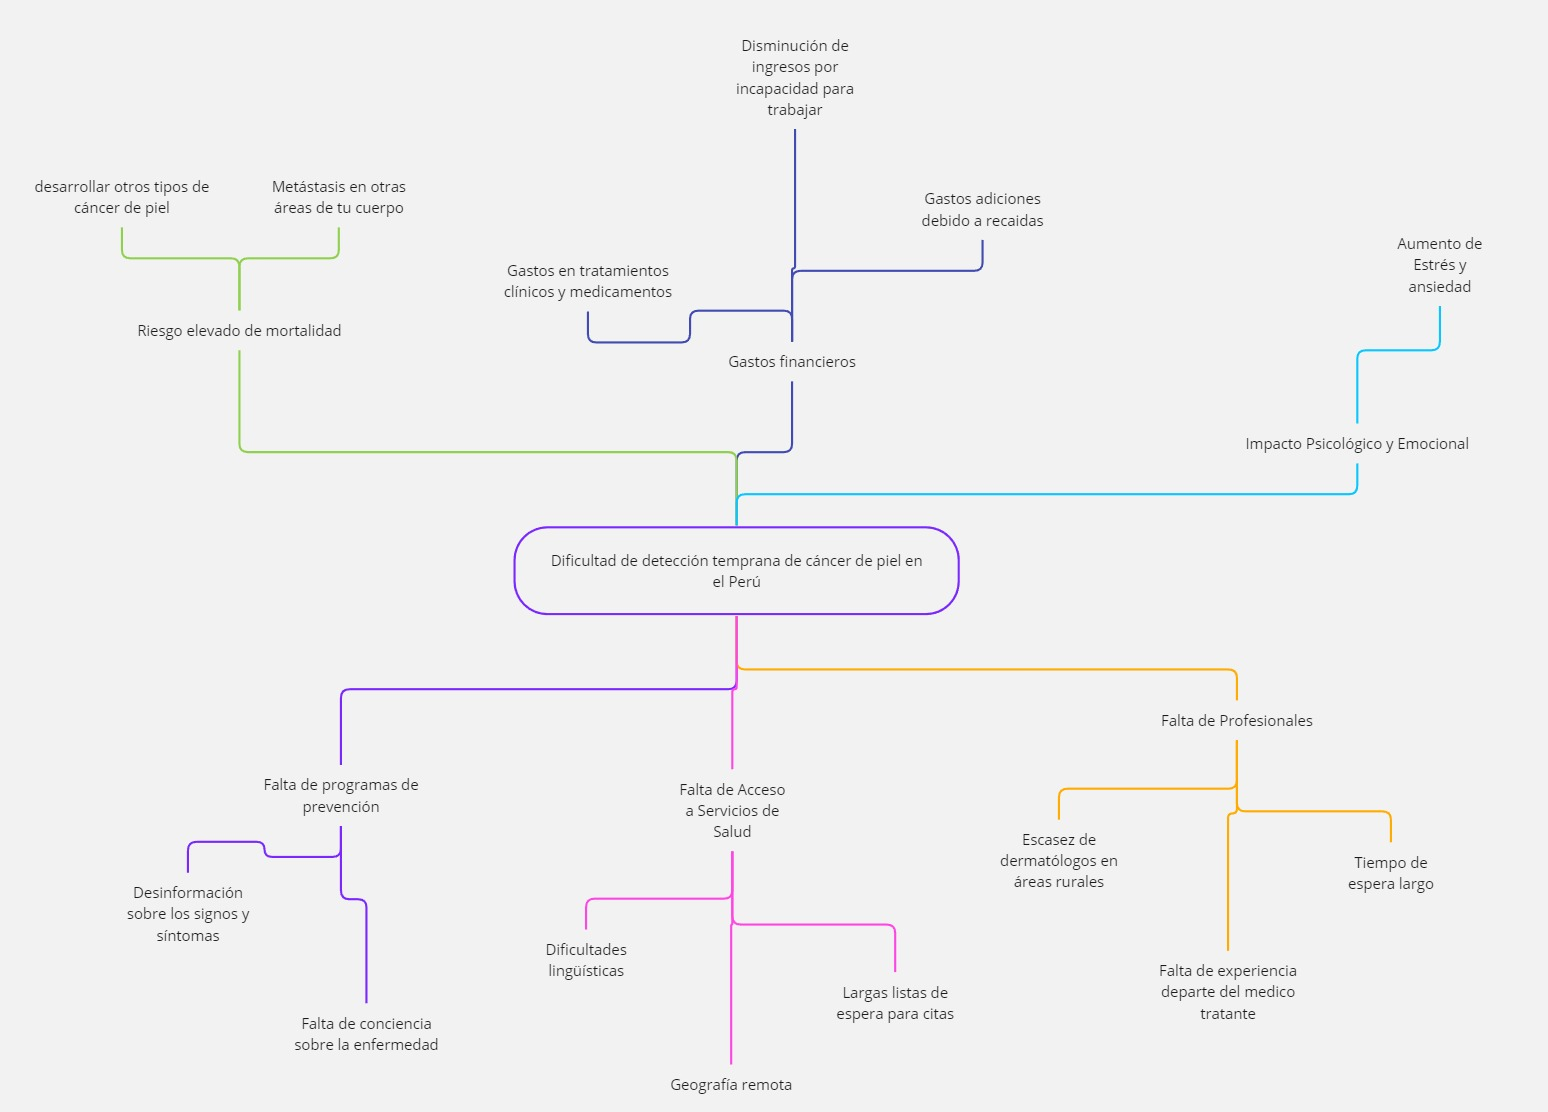
\includegraphics[width=0.8\textwidth]{images_repo/Anexo/Problem Tree Template.jpg}
		\caption{Árbol de Problema. Fuente: Elaboración propia}
		\label{1:arbolProblema}
	\end{center}
\end{figure}



\chapter{Anexo II: Árbol de Objetivo}

\begin{figure}[h]
	\begin{center}
		\includegraphics[width=0.8\textwidth]{images_repo/Anexo/Árbol de Objetivos.jpg}
		\caption{Árbol de Problema. Fuente: Elaboración propia}
		\label{1:arbolObjeti}
	\end{center}
\end{figure}



\chapter{Anexo II: Matriz de Consistencia}


\begin{table}[h!]
	\centering
	\small
	\begin{tabular}{ |m{5cm}|m{5cm}|m{5cm}|  }
		\hline
		\rowcolor{bluejean}
		\Centering \color{white}{PROBLEMAS}& \Centering \color{white}{OBJETIVOS}& \Centering \color{white}{HIPÓTESIS}\\
		\hline
		\rowcolor{turq}
		\Centering Problema General& \Centering Objetivo General & \Centering Hipótesis General \\
		\hline
		{\ProblemaGeneral} & { \ObjetivoGeneral} & {\HipotesisGeneral} \\
		\hline
		\rowcolor{turq}
		\Centering Problemas Específicos& \Centering Objetivos Específicos & \Centering Hipótesis Específicas \\
		\hline
		{\Pbone} & {\Objone} & {\Hone} \\
		\hline
		{\Pbtwo} & {\Objtwo} & {\Htwo} \\
		\hline
		{\Pbthree} & {\Objthree} & {\Hthree} \\
		\hline
		{\Pbfour} & {\Objfour} & {\Hfour} \\
		\hline
		{\Pbfive} & {\Objfive} & {\Hfive} \\
		\hline
	\end{tabular}
	\caption{Matriz de consistencia. Fuente: Elaboración propia}
	\label{1:table}
\end{table}



\chapter{Anexo II: Resumen de Papers investigados}
%\section{Conclusiones}

\begin{table}[h]
	\newcommand{\multirot}[1]{\multirow{2}{*}[-8ex]{\rotcell{\rlap{#1}}}}
	%\scriptsize
	\footnotesize
	\centering
	\begin{tabular}{|m{0.5cm}|m{0.3cm}|m{4cm}|m{2cm}|m{0.6cm}|m{1.7cm}|m{3cm}|} 
		\hline
		\rowcolor[rgb]{0,0.251,0.502} \multicolumn{1}{|c|}{\textcolor{white}{Tipo}} & \multicolumn{1}{c|}{\textcolor{white}{N°}} & \multicolumn{1}{c|}{\textcolor{white}{Título}}                                                                             & \multicolumn{1}{c|}{\textcolor{white}{Autor}}        & \multicolumn{1}{c|}{\textcolor{white}{Año}} & \multicolumn{1}{c|}{\textcolor{white}{País}} & \multicolumn{1}{c|}{\textcolor{white}{Fuente}}                                                        \\ 
		\hline
		\multirot{Problema}                                        & 1                                             & Deep Learning-Based Transfer Learning for Classification of Skin Cancer~                                                                               & Satin, J. , Udit, S., Balakrushna, T., Emad, A. Mohamed K. and Ali K. & 2021 &  Arabia Saudita. & Sensors \\ 
		\cline{2-7}
		& 2                                             & Skin cancer classification via convolutional neural networks: systematic review of studies involving human experts                                                          & S. Haggenmu ̈ller, A. Hekler, R.C. Maron,  (...) ,  V.M. Rotemberg                 & 2021                                        & Europa                                 & European Journal of Cancer                                                \\ 
		\hline
		\multirow{3}{*}[-14ex]{\rotcell{\rlap{Propuesta}}}
		& 3                                             & An enhanced technique of skin cancer classification using deep convolutional neural network with transfer learning models~                                                                               & Md Shahin Ali, Md Sipon Miah, Jahurul Haque, Md Mahbubur Rahman y Md Khairul Islam                                 & 2021                                        &  República de Irlanda         & Machine Learning with Applications, 2021, vol. 5                                                                  \\ 
		\cline{2-7}
		& 4                                             & Design of a tool for the classification of skin cancer imagesusing Deep Neural Networks (DNN)~                                                                                & Diana Paola Merchán Vargas, Helis Navarro Báez, Jaime Guillermo Barrero Pérez y Jeyson Arley Castillo Bohórquez                                          & 2021                                        & Argentina                                          & "Ciencia y Tecnología", número 21 del año 2021.                                                            \\ 
		
	     \hline
		\multirow{4}{*}[-28ex]{\rotcell{\rlap{Técnica}}}                                          
			& 5                                             & Diagnosis of skin cancer using machine learning techniques                                               &A. Murugan, S. Anu H. Nair y K.P. Sanal Kumar & 2021                                        & India                                          & Microprocessors and Microsystems en 2021             \\ 
		\cline{2-7}
		
		
		
		
		& 6                                             & Multiclass skin cancer classification using EfficientNets – a first step towards preventing skin cancer~                   & K. Ali, Z.A. Shaikh, A.A. Khan, S. Rathod, S. Das                                      & 2022                                        & Pakistan                                        & 2022, revista Neuroscience Informatics \\ 
		\cline{2-7}
		& 7                                             & Skin cancer classification using explainable artificial intelligence on pre-extracted image features & Khater, T., Ansari, S., Mahmoud, S., Hussain, A., Tawfik, H. & 2017 & Miratos Árabes Unidos          & revista "Intelligent Systems with Applications" en el año 2023
		Association of Automation (YAC)~              \\ 
		\cline{2-7}
		& 8                                             & An improved transformer network for skin cancer classification
		 &  C. Xin, Y. Wang, G. Wang, X. Zhao, Y. Dong y M. Lu.~             & 2022                                        & China                                          & Computers in Biology and Medicine              \\ 
		\cline{2-7}
		& 9                                             & Uncertainty quantification in skin cancer classification using three-way decision-based Bayesian deep learning                                                                      & M. Abdar, F. Pourpanah, S. Hussain, D. Rezazadegan, L. Liu, M. Ghavamzadeh, P. Fieguth, X. Cao, A. Khosravi y U.R. Acharya                                   & 2021                                        & -                                          & Computers in Biology and Medicine                          \\
		\cline{2-7}
		& 10                                             &A multi-class skin Cancer classification using deep convolutional neural networks    & Saket S. Chaturvedi, Jitendra V. Tembhurne, Tausif Diwan2 & 2020                               & -         & Springer Science+Business Media, LLC, part of Springer Nature 2020 \\
		\hline
	\end{tabular}
	\caption{Cuadro Resumen de Papers investigados. Fuente: Elaboración propia}
\label{A:table}
\end{table}




